% !TeX spellcheck = en_US
% !TeX root = notes.tex
\subsection{Application Layer}
% HTTP request, reply
\subsubsection{Request Message}
\begin{figure}[H]
	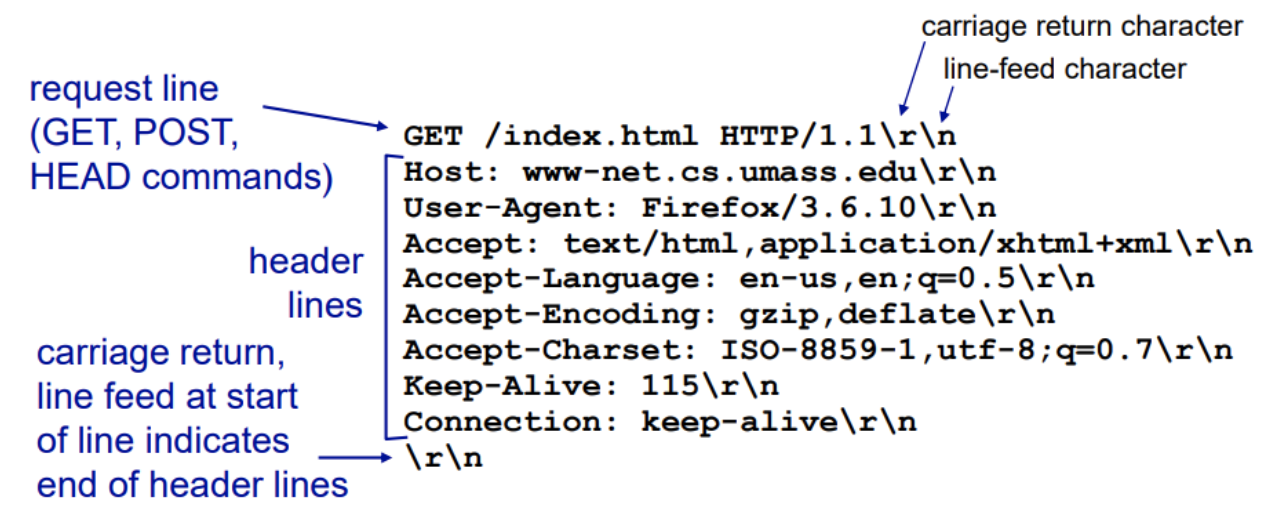
\includegraphics[width=\linewidth]{request}
	\centering
	\caption{HTTP Request Message}
\end{figure}
\subsubsection{Response Message}
\begin{figure}[H]
	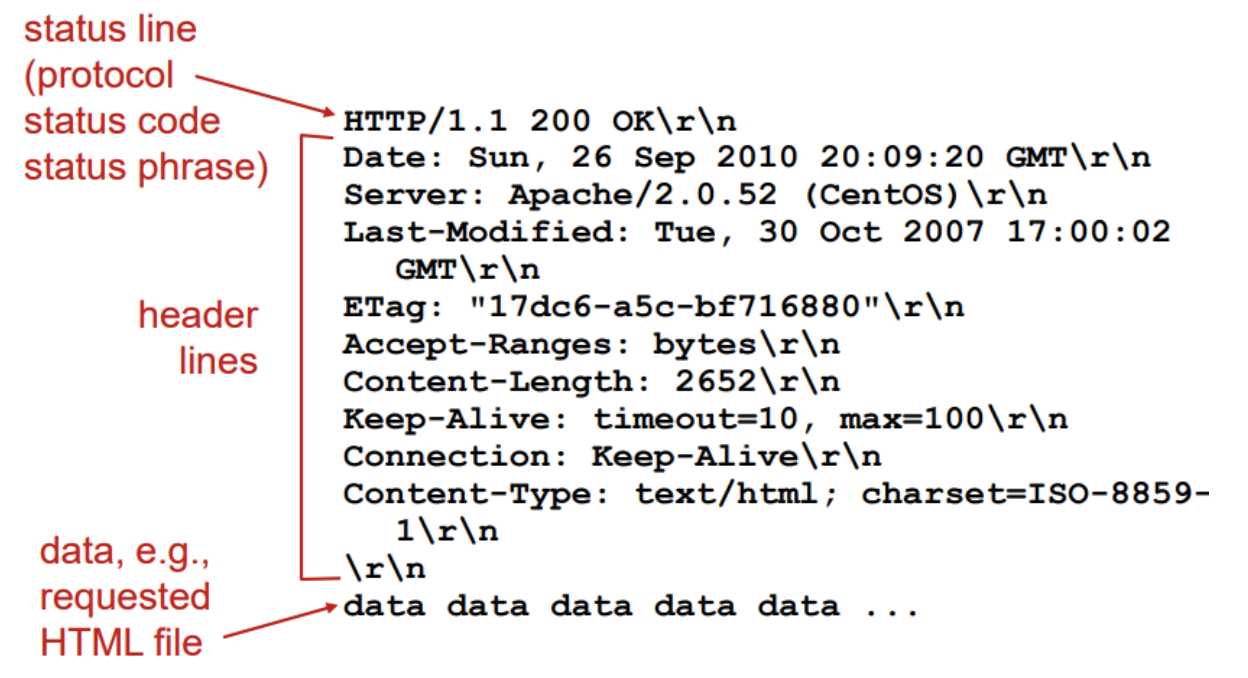
\includegraphics[width=\linewidth]{response}
	\centering
	\caption{HTTP Response Message}
\end{figure}

\subsection{Presentation}
\textbf{ISO/OSI Reference:} Allow applications to interpret meaning of data, e.g. encryption, compression, machine-specific conventions
\subsection{Session}
\textbf{ISO/OSI Reference:} Synchronization, check-pointing, recovery of data exchange

\subsection{Transport Layer}
% TCP, UDP
\subsubsection{UDP}
\begin{table}[H]
	\centering
	\caption{UDP Breakdown}
	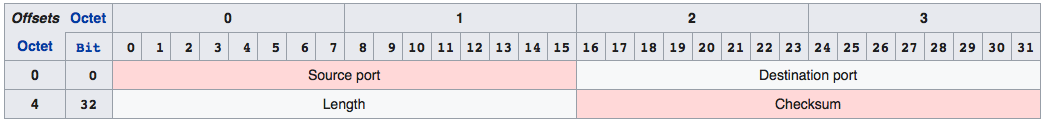
\includegraphics[width=\linewidth]{udp}
\end{table}
\begin{description}
	\item[Source Port:] Sender's port number
	\item[Destination Port:] Receiver's port number
	\item[Length:] Length of UDP header and data in bytes. Min is 8, max is 65,535 bytes
	\item[Checksum:] Optional for IPv4
\end{description}
\subsubsection{TCP}
\begin{table}[H]
	\centering
	\caption{TCP Breakdown}
	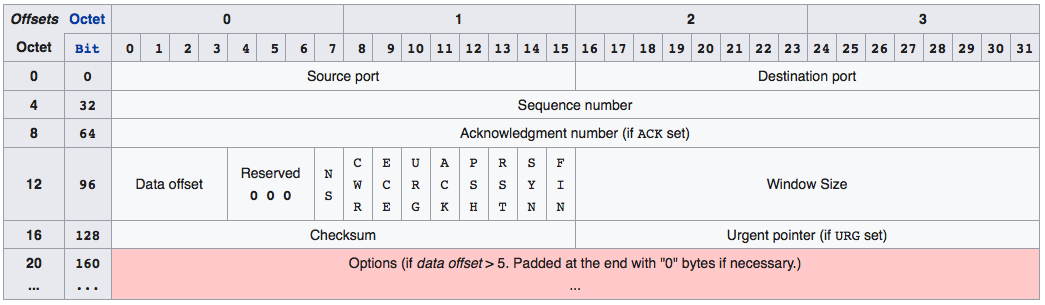
\includegraphics[width=\linewidth]{tcp}
\end{table}
\begin{description}
	\item[Source Port:] Sending Port
	\item[Destination Port:] Receiving Port
	\item[Sequence Number:] If the \texttt{SYN} flag is set (1), then this is the initial sequence number. The sequence number of the actual first data byte and the acknowledged number in the corresponding ACK are then this sequence number plus 1
	\subitem If the \texttt{SYN} flag is clear (0), then this is the accumulated sequence number of the first data byte of this segment for the current session
	\item[Acknowledgment number:] If the \texttt{ACK} flag is set then the value of this field is the next sequence number that the sender of the ACK is expecting. This acknowledges receipt of all prior bytes (if any). The first \texttt{ACK} sent by each end acknowledges the other end's initial sequence number itself, but no data
	\item[Data offset:] Size of TCP header in 32-bit words. Min 5, Max 15 words (max of 60 bytes $\rightarrow$ 40 byte options)
	\item[Flags:]
	\begin{description}
		\item[NS:] ECN-nonce concealment
		\item[CWR:] Congestion Window Reduction
		\item[ECE:] ECN-Echo
		\item[URG:] Urgent pointer field is significant
		\item[ACK:] Acknowledgment field is significant
		\item[PSH:] Push function
		\item[RST:] Reset the connection
		\item[SYN:] Synchronize sequence numbers
		\item[FIN:] Last packet from sender
	\end{description}
	\item[Window Size:] Number of bytes the receiver is currently willing to accept
	\item[Checksum:] Error-checking of header, payload, and Pseudo-Header. Pseudo-Header includes; Source IP Address, Destination IP Address, protocol number (typically 0x0006), and length of TCP-Headers including payload
	\item[Urgent Pointer:] Offset from sequence number indicating last urgent data byte (if \texttt{URG} set (1))
	\item[Options:] \textit{Pray to god this doesn't show up on the exam}
\end{description}

\subsection{Network Layer}
% IPv4, ICMP, DNS
\subsubsection{IPv4}
\begin{table}[H]
	\centering
	\caption{IPv4 Breakdown}
	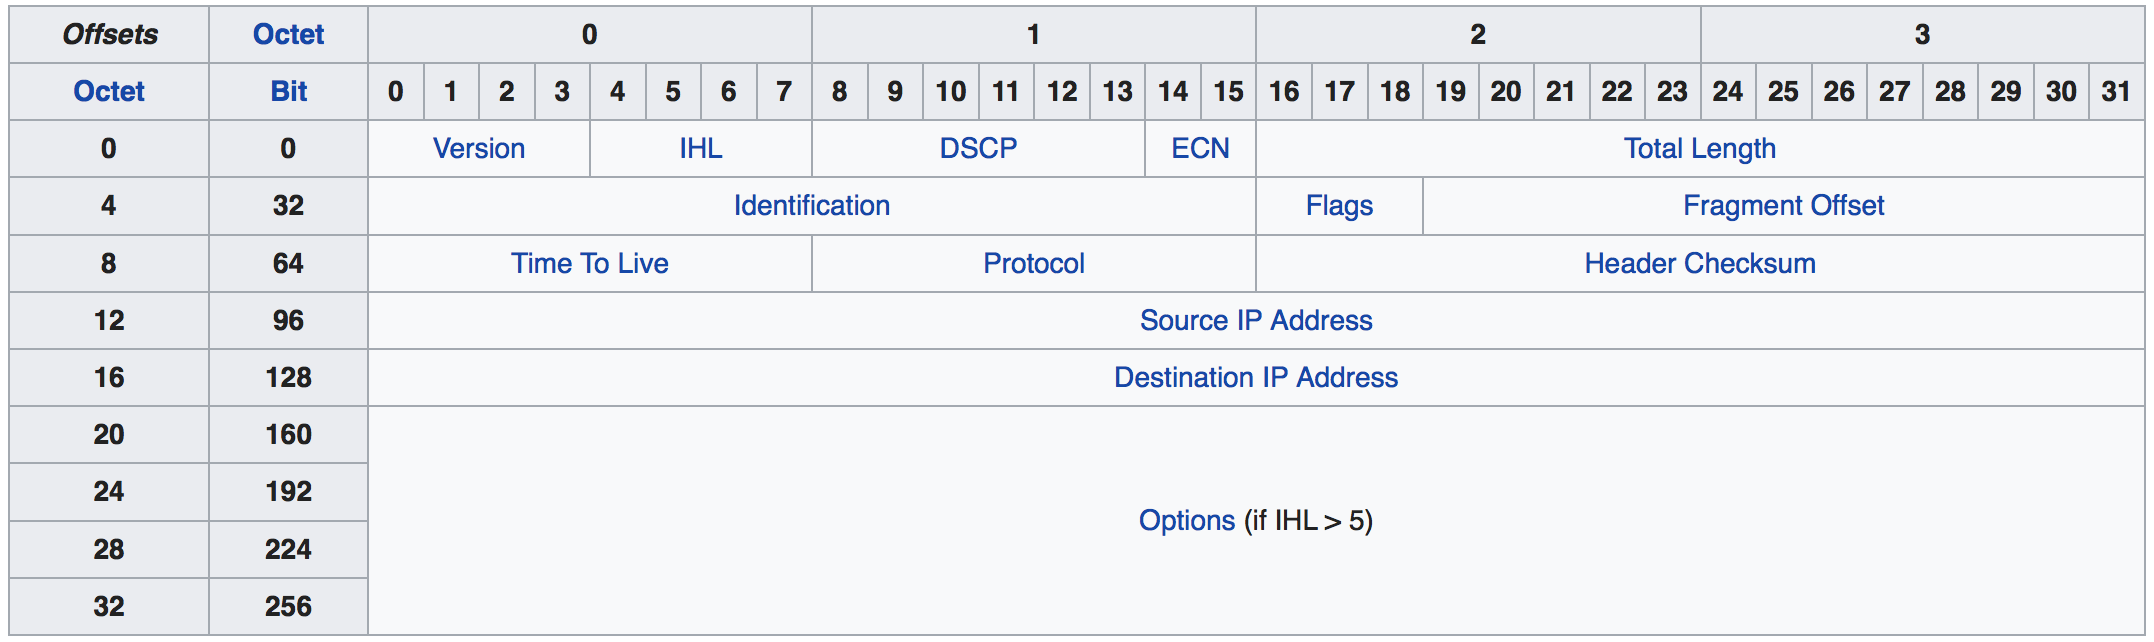
\includegraphics[width=\linewidth]{ipv4}
\end{table}
\begin{description}
	\item[Version:] For IPv4, this is always 4
	\item[Internet Header Length(IHL):] Length of the header times 4 (e.g. IHL = 5, header length is $5\times4=20$ bytes. Minimum value is $5$, max is $15$
	\item[Differentiated Services Code Point (DSCP):] Originally ToS, used for DiffServ technologies requiring real-time streaming (e.g. VoIP)
	\item[Explicit Congestion Notification (ECN):] Notifies each end of congestion without dropping packets
	\item[Total Length:] Entire packet size, including header and data. Min is 20, max is 65,535 bytes
	\item[Identification:] Helps identify groups of IP packets that have been fragmented
	\item[Flags:] bit 0: Reserved, must be zero. bit 1: Don't Fragment (DF). bit 2: More Fragments (MF)
	\item[Fragment Offset:] Measured in 8-byte blocks, provides the offset since the original unfragmented IP datagram
	\item[Time To Live (TTL):] Used to make sure the packet doesn't stay in circulation on the Internet
	\item[Protocol:] See Table~\ref{fig:protocols}. If port 53 and protocol is UDP, DNS request most likely
	\item[Header Checksum:] Checksum for the header only, encapsulated protocol must handle incorrect data errors
	\item[Source Address:] IPv4 sender address for the packet
	\item[Destination Address:] IPv4 receiver address for the packet
	\item[Options:] Options field not often used. IHL must include enough width to allocate for options. Options can end with an EOL (End of Options List, 0x00) if it doesn't match up with ending of IHL. Possible options are:
	\begin{description}
		\item[Copied:] (1 bit) Set to 1 if the options need to be copied into all fragments of a fragmented packet
		\item[Option Class:] (2 bits) A general options category. 0 is for ``control'' options, and 2 is for ``debugging and measurement''. 1 and 3 reserved
		\item[Option Number:] (5 bits) Specifies an option
		\item[Option Length:] (8 bits) Indicated the size of the entire option (including this field). This field may not exist for simple options
		\item[Option Data:] (Variable Bits) Option-specific data. This field may not exist for simple options
	\end{description}
\end{description}
\begin{table}[H]
	\centering
	\caption{Internet Protocol Numbers from RFC 790}\label{fig:protocols}
	\begin{tabular}{rrl}
	\toprule
	Decimal & Hex & Protocol\\
	\midrule
	1 && Internet Control Message Protocol (ICMP)\\
	2 && Internet Group Management Protocol (IGMP)\\
	6 && Transmission Control Protocol (TCP)\\
	17 && User Datagram Protocol (UDP)\\
	41 && IPv6 encapsulation (ENCAP)\\
	89 && Open Shortest Path First (OSPF)\\
	132 && Stream Control Transmission Protocol (SCTP)\\
	\bottomrule
	\end{tabular}
\end{table}

\subsection{Link Layer}
% Ethernet
\begin{figure}[H]
	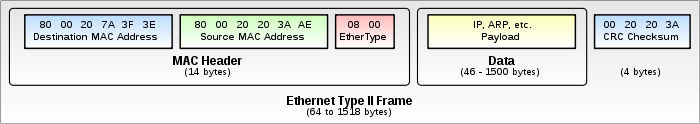
\includegraphics[width=\linewidth]{ethernet}
	\centering
	\caption{Ethernet Breakdown}
\end{figure}
\begin{description}
	\item[Destination:] (6 bytes) Destination MAC Address
	\item[Source:] (6 bytes) Source MAC Address
	\item[Type:] (2 bytes) The type of internet communication (IPv4: 0x0800)
\end{description}
\subsection{Physical}
% Nothing mentioned, just get stuff from notes